\documentclass{standalone}
\usepackage{tikz}
\usetikzlibrary{patterns, positioning}


\begin{document}
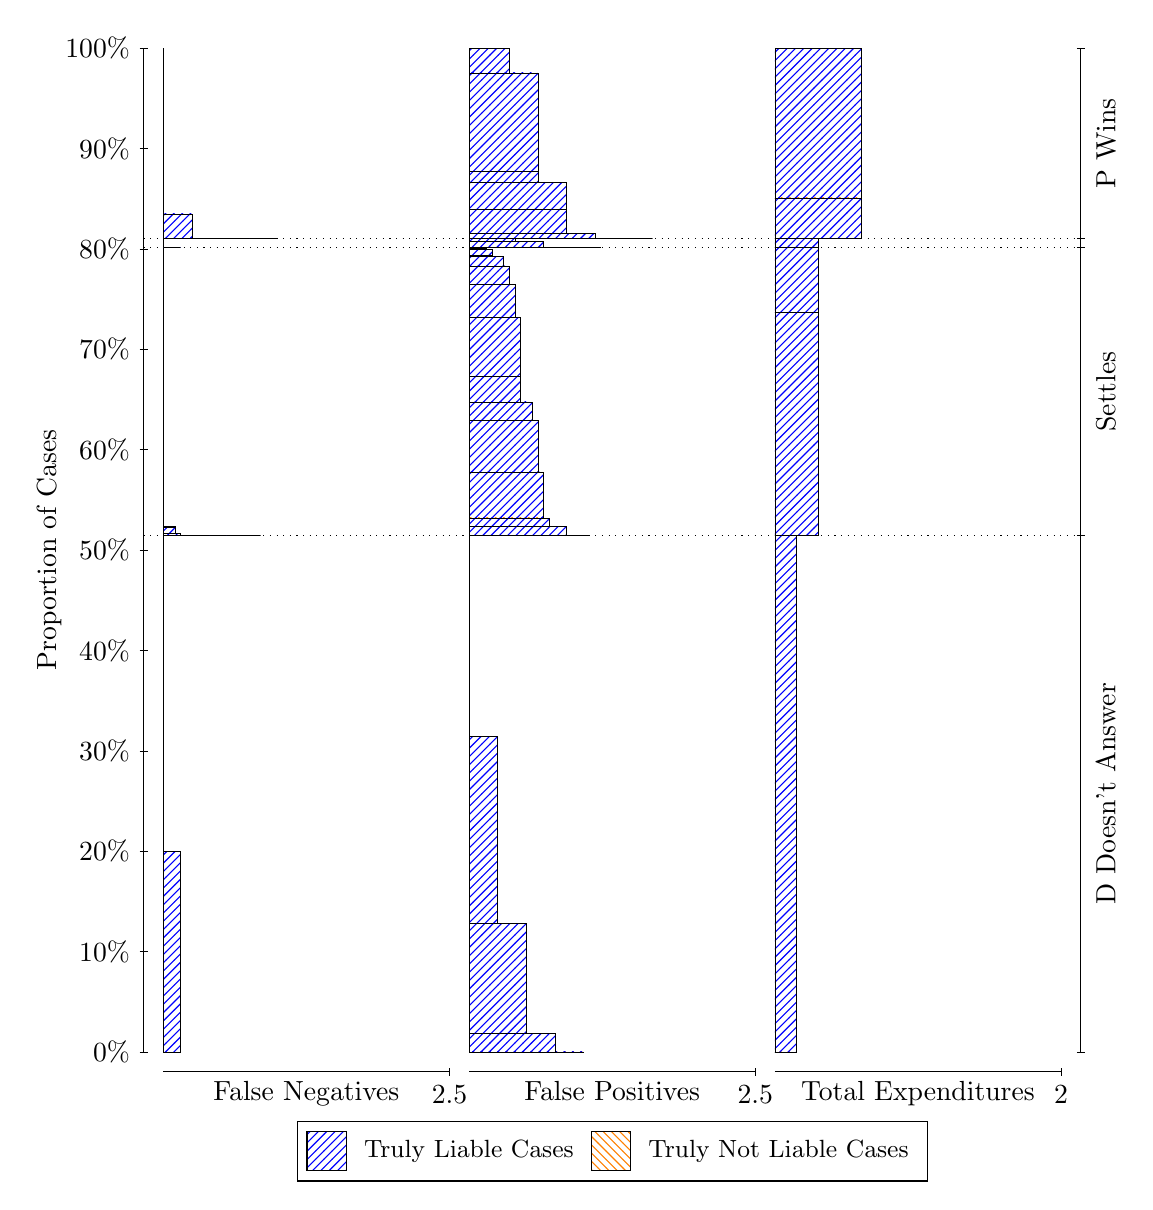
\begin{tikzpicture}
\draw[black, very thin] (1.5,1.75) -- (1.5,14.5);
\node[rotate=90, text=black, anchor=center] at (0.3, 8.125) {Proportion of Cases};
\draw[black, very thin] (1.45,1.75) -- (1.55,1.75);
\node[text=black, anchor=east] at (1.45, 1.75) {0\%};
\draw[black, very thin] (1.45,3.025) -- (1.55,3.025);
\node[text=black, anchor=east] at (1.45, 3.025) {10\%};
\draw[black, very thin] (1.45,4.3) -- (1.55,4.3);
\node[text=black, anchor=east] at (1.45, 4.3) {20\%};
\draw[black, very thin] (1.45,5.575) -- (1.55,5.575);
\node[text=black, anchor=east] at (1.45, 5.575) {30\%};
\draw[black, very thin] (1.45,6.85) -- (1.55,6.85);
\node[text=black, anchor=east] at (1.45, 6.85) {40\%};
\draw[black, very thin] (1.45,8.125) -- (1.55,8.125);
\node[text=black, anchor=east] at (1.45, 8.125) {50\%};
\draw[black, very thin] (1.45,9.4) -- (1.55,9.4);
\node[text=black, anchor=east] at (1.45, 9.4) {60\%};
\draw[black, very thin] (1.45,10.675) -- (1.55,10.675);
\node[text=black, anchor=east] at (1.45, 10.675) {70\%};
\draw[black, very thin] (1.45,11.95) -- (1.55,11.95);
\node[text=black, anchor=east] at (1.45, 11.95) {80\%};
\draw[black, very thin] (1.45,13.225) -- (1.55,13.225);
\node[text=black, anchor=east] at (1.45, 13.225) {90\%};
\draw[black, very thin] (1.45,14.5) -- (1.55,14.5);
\node[text=black, anchor=east] at (1.45, 14.5) {100\%};

\draw[black, very thin] (13.4,1.75) -- (13.4,14.5);
\draw[black, very thin] (13.35,1.75) -- (13.45,1.75);
\node[anchor=west] at (13.35, 1.75) {};
\draw[black, very thin] (13.35,8.3072) -- (13.45,8.3072);
\node[anchor=west] at (13.35, 8.3072) {};
\draw[black, very thin] (13.35,11.968) -- (13.45,11.968);
\node[anchor=west] at (13.35, 11.968) {};
\draw[black, very thin] (13.35,12.079) -- (13.45,12.079);
\node[anchor=west] at (13.35, 12.079) {};
\draw[black, very thin] (13.35,14.5) -- (13.45,14.5);
\node[anchor=west] at (13.35, 14.5) {};

\draw[black, very thin, pattern color=blue, pattern=north east lines] (1.75,1.75) rectangle (1.968,4.2982);
\draw[black, very thin, pattern color=orange, pattern=north west lines] (1.75,4.2982) rectangle (1.75,4.2982);
\draw[black, very thin, pattern color=blue, pattern=north east lines] (1.75,4.2982) rectangle (1.75,8.3072);
\draw[black, very thin, pattern color=blue, pattern=north east lines] (1.75,8.3072) rectangle (2.9853,8.3072);
\draw[black, very thin, pattern color=blue, pattern=north east lines] (1.75,8.3072) rectangle (2.6947,8.3072);
\draw[black, very thin, pattern color=blue, pattern=north east lines] (1.75,8.3072) rectangle (2.622,8.3072);
\draw[black, very thin, pattern color=blue, pattern=north east lines] (1.75,8.3072) rectangle (2.5493,8.3072);
\draw[black, very thin, pattern color=blue, pattern=north east lines] (1.75,8.3072) rectangle (2.404,8.3072);
\draw[black, very thin, pattern color=blue, pattern=north east lines] (1.75,8.3072) rectangle (2.3313,8.3072);
\draw[black, very thin, pattern color=blue, pattern=north east lines] (1.75,8.3072) rectangle (2.2587,8.3073);
\draw[black, very thin, pattern color=blue, pattern=north east lines] (1.75,8.3073) rectangle (2.186,8.3073);
\draw[black, very thin, pattern color=blue, pattern=north east lines] (1.75,8.3073) rectangle (2.1133,8.3086);
\draw[black, very thin, pattern color=blue, pattern=north east lines] (1.75,8.3086) rectangle (2.0407,8.3138);
\draw[black, very thin, pattern color=blue, pattern=north east lines] (1.75,8.3138) rectangle (1.968,8.3318);
\draw[black, very thin, pattern color=blue, pattern=north east lines] (1.75,8.3318) rectangle (1.8953,8.4121);
\draw[black, very thin, pattern color=blue, pattern=north east lines] (1.75,8.4121) rectangle (1.8953,8.425);
\draw[black, very thin, pattern color=blue, pattern=north east lines] (1.75,8.425) rectangle (1.8227,8.4254);
\draw[black, very thin, pattern color=orange, pattern=north west lines] (1.75,8.4254) rectangle (1.75,8.4254);
\draw[black, very thin, pattern color=blue, pattern=north east lines] (1.75,8.4254) rectangle (1.75,11.968);
\draw[black, very thin, pattern color=blue, pattern=north east lines] (1.75,11.968) rectangle (1.968,11.968);
\draw[black, very thin, pattern color=orange, pattern=north west lines] (1.75,11.968) rectangle (1.75,11.968);
\draw[black, very thin, pattern color=blue, pattern=north east lines] (1.75,11.968) rectangle (1.75,12.079);
\draw[black, very thin, pattern color=blue, pattern=north east lines] (1.75,12.079) rectangle (3.2033,12.079);
\draw[black, very thin, pattern color=blue, pattern=north east lines] (1.75,12.079) rectangle (2.84,12.079);
\draw[black, very thin, pattern color=blue, pattern=north east lines] (1.75,12.079) rectangle (2.4767,12.085);
\draw[black, very thin, pattern color=blue, pattern=north east lines] (1.75,12.085) rectangle (2.1133,12.395);
\draw[black, very thin, pattern color=orange, pattern=north west lines] (1.75,12.395) rectangle (1.75,12.395);
\draw[black, very thin, pattern color=blue, pattern=north east lines] (1.75,12.395) rectangle (1.75,14.5);
\draw[black, very thin, pattern color=orange, pattern=north west lines] (5.6333,1.75) rectangle (7.0867,1.75);
\draw[black, very thin, pattern color=blue, pattern=north east lines] (5.6333,1.75) rectangle (7.0867,1.7523);
\draw[black, very thin, pattern color=blue, pattern=north east lines] (5.6333,1.7523) rectangle (6.7233,1.9853);
\draw[black, very thin, pattern color=blue, pattern=north east lines] (5.6333,1.9853) rectangle (6.36,3.3846);
\draw[black, very thin, pattern color=blue, pattern=north east lines] (5.6333,3.3846) rectangle (5.9967,5.759);
\draw[black, very thin, pattern color=blue, pattern=north east lines] (5.6333,5.759) rectangle (5.6333,8.3072);
\draw[black, very thin, pattern color=orange, pattern=north west lines] (5.6333,8.3072) rectangle (7.1593,8.3072);
\draw[black, very thin, pattern color=blue, pattern=north east lines] (5.6333,8.3072) rectangle (7.1593,8.3072);
\draw[black, very thin, pattern color=orange, pattern=north west lines] (5.6333,8.3072) rectangle (7.014,8.3072);
\draw[black, very thin, pattern color=blue, pattern=north east lines] (5.6333,8.3072) rectangle (7.014,8.3079);
\draw[black, very thin, pattern color=orange, pattern=north west lines] (5.6333,8.3079) rectangle (6.8687,8.3079);
\draw[black, very thin, pattern color=blue, pattern=north east lines] (5.6333,8.3079) rectangle (6.8687,8.4215);
\draw[black, very thin, pattern color=blue, pattern=north east lines] (5.6333,8.4215) rectangle (6.796,8.429);
\draw[black, very thin, pattern color=orange, pattern=north west lines] (5.6333,8.429) rectangle (6.7233,8.429);
\draw[black, very thin, pattern color=blue, pattern=north east lines] (5.6333,8.429) rectangle (6.7233,8.4295);
\draw[black, very thin, pattern color=blue, pattern=north east lines] (5.6333,8.4295) rectangle (6.6507,8.5315);
\draw[black, very thin, pattern color=orange, pattern=north west lines] (5.6333,8.5315) rectangle (6.578,8.5315);
\draw[black, very thin, pattern color=blue, pattern=north east lines] (5.6333,8.5315) rectangle (6.578,9.1175);
\draw[black, very thin, pattern color=blue, pattern=north east lines] (5.6333,9.1175) rectangle (6.5053,9.7733);
\draw[black, very thin, pattern color=blue, pattern=north east lines] (5.6333,9.7733) rectangle (6.4327,9.9982);
\draw[black, very thin, pattern color=blue, pattern=north east lines] (5.6333,9.9982) rectangle (6.36,10.007);
\draw[black, very thin, pattern color=blue, pattern=north east lines] (5.6333,10.007) rectangle (6.2873,10.328);
\draw[black, very thin, pattern color=orange, pattern=north west lines] (5.6333,10.328) rectangle (6.2873,10.328);
\draw[black, very thin, pattern color=blue, pattern=north east lines] (5.6333,10.328) rectangle (6.2873,11.077);
\draw[black, very thin, pattern color=blue, pattern=north east lines] (5.6333,11.077) rectangle (6.2147,11.502);
\draw[black, very thin, pattern color=blue, pattern=north east lines] (5.6333,11.502) rectangle (6.142,11.734);
\draw[black, very thin, pattern color=blue, pattern=north east lines] (5.6333,11.734) rectangle (6.0693,11.85);
\draw[black, very thin, pattern color=blue, pattern=north east lines] (5.6333,11.85) rectangle (5.9967,11.85);
\draw[black, very thin, pattern color=blue, pattern=north east lines] (5.6333,11.85) rectangle (5.924,11.863);
\draw[black, very thin, pattern color=blue, pattern=north east lines] (5.6333,11.863) rectangle (5.924,11.943);
\draw[black, very thin, pattern color=blue, pattern=north east lines] (5.6333,11.943) rectangle (5.8513,11.961);
\draw[black, very thin, pattern color=blue, pattern=north east lines] (5.6333,11.961) rectangle (5.7787,11.967);
\draw[black, very thin, pattern color=blue, pattern=north east lines] (5.6333,11.967) rectangle (5.706,11.968);
\draw[black, very thin, pattern color=blue, pattern=north east lines] (5.6333,11.968) rectangle (5.6333,11.968);
\draw[black, very thin, pattern color=orange, pattern=north west lines] (5.6333,11.968) rectangle (7.3047,11.968);
\draw[black, very thin, pattern color=blue, pattern=north east lines] (5.6333,11.968) rectangle (7.3047,11.968);
\draw[black, very thin, pattern color=blue, pattern=north east lines] (5.6333,11.968) rectangle (6.9413,11.97);
\draw[black, very thin, pattern color=blue, pattern=north east lines] (5.6333,11.97) rectangle (6.578,12.04);
\draw[black, very thin, pattern color=blue, pattern=north east lines] (5.6333,12.04) rectangle (6.2147,12.078);
\draw[black, very thin, pattern color=blue, pattern=north east lines] (5.6333,12.078) rectangle (5.8513,12.079);
\draw[black, very thin, pattern color=orange, pattern=north west lines] (5.6333,12.079) rectangle (7.9587,12.079);
\draw[black, very thin, pattern color=blue, pattern=north east lines] (5.6333,12.079) rectangle (7.9587,12.079);
\draw[black, very thin, pattern color=orange, pattern=north west lines] (5.6333,12.079) rectangle (7.5953,12.079);
\draw[black, very thin, pattern color=blue, pattern=north east lines] (5.6333,12.079) rectangle (7.5953,12.08);
\draw[black, very thin, pattern color=orange, pattern=north west lines] (5.6333,12.08) rectangle (7.232,12.08);
\draw[black, very thin, pattern color=blue, pattern=north east lines] (5.6333,12.08) rectangle (7.232,12.143);
\draw[black, very thin, pattern color=blue, pattern=north east lines] (5.6333,12.143) rectangle (6.8687,12.452);
\draw[black, very thin, pattern color=orange, pattern=north west lines] (5.6333,12.452) rectangle (6.8687,12.452);
\draw[black, very thin, pattern color=blue, pattern=north east lines] (5.6333,12.452) rectangle (6.8687,12.79);
\draw[black, very thin, pattern color=blue, pattern=north east lines] (5.6333,12.79) rectangle (6.5053,12.933);
\draw[black, very thin, pattern color=orange, pattern=north west lines] (5.6333,12.933) rectangle (6.5053,12.933);
\draw[black, very thin, pattern color=blue, pattern=north east lines] (5.6333,12.933) rectangle (6.5053,14.184);
\draw[black, very thin, pattern color=blue, pattern=north east lines] (5.6333,14.184) rectangle (6.142,14.185);
\draw[black, very thin, pattern color=blue, pattern=north east lines] (5.6333,14.185) rectangle (6.142,14.494);
\draw[black, very thin, pattern color=blue, pattern=north east lines] (5.6333,14.494) rectangle (5.7787,14.494);
\draw[black, very thin, pattern color=blue, pattern=north east lines] (5.6333,14.494) rectangle (5.7787,14.5);
\draw[black, very thin, pattern color=blue, pattern=north east lines] (5.6333,14.5) rectangle (5.6333,14.5);
\draw[black, very thin, pattern color=orange, pattern=north west lines] (9.5167,1.75) rectangle (9.7892,1.75);
\draw[black, very thin, pattern color=blue, pattern=north east lines] (9.5167,1.75) rectangle (9.7892,8.3072);
\draw[black, very thin, pattern color=orange, pattern=north west lines] (9.5167,8.3072) rectangle (10.062,8.3072);
\draw[black, very thin, pattern color=blue, pattern=north east lines] (9.5167,8.3072) rectangle (10.062,11.139);
\draw[black, very thin, pattern color=orange, pattern=north west lines] (9.5167,11.139) rectangle (10.062,11.139);
\draw[black, very thin, pattern color=blue, pattern=north east lines] (9.5167,11.139) rectangle (10.062,11.968);
\draw[black, very thin, pattern color=orange, pattern=north west lines] (9.5167,11.968) rectangle (10.062,11.968);
\draw[black, very thin, pattern color=blue, pattern=north east lines] (9.5167,11.968) rectangle (10.062,12.079);
\draw[black, very thin, pattern color=orange, pattern=north west lines] (9.5167,12.079) rectangle (10.607,12.079);
\draw[black, very thin, pattern color=blue, pattern=north east lines] (9.5167,12.079) rectangle (10.607,12.596);
\draw[black, very thin, pattern color=orange, pattern=north west lines] (9.5167,12.596) rectangle (10.607,12.596);
\draw[black, very thin, pattern color=blue, pattern=north east lines] (9.5167,12.596) rectangle (10.607,14.5);
\draw[black, dotted] (1.5,8.3072) -- (13.4,8.3072);
\draw[black, dotted] (1.5,11.968) -- (13.4,11.968);
\draw[black, dotted] (1.5,12.079) -- (13.4,12.079);
\draw[black, very thin] (1.75,1.5) -- (5.3833,1.5);
\node[text=black, anchor=north] at (3.5667, 1.5) {False Negatives};
\draw[black, very thin] (5.3833,1.45) -- (5.3833,1.55);
\node[text=black, anchor=north] at (5.3833, 1.45) {2.5};

\draw[black, very thin] (5.6333,1.5) -- (9.2667,1.5);
\node[text=black, anchor=north] at (7.45, 1.5) {False Positives};
\draw[black, very thin] (9.2667,1.45) -- (9.2667,1.55);
\node[text=black, anchor=north] at (9.2667, 1.45) {2.5};

\draw[black, very thin] (9.5167,1.5) -- (13.15,1.5);
\node[text=black, anchor=north] at (11.333, 1.5) {Total Expenditures};
\draw[black, very thin] (13.15,1.45) -- (13.15,1.55);
\node[text=black, anchor=north] at (13.15, 1.45) {2};

\node[text=black, centered, rotate=90] at (13.72, 5.0286) {D Doesn't Answer};
\node[text=black, centered, rotate=90] at (13.72, 10.138) {Settles};

\node[text=black, centered, rotate=90] at (13.72, 13.289) {P Wins};

\draw (7.449999999999999,1.5) node[draw=none] (baseCoordinate) {};
\begin{scope}[align=center]
        \matrix[scale=0.5, draw=black, below=0.5cm of baseCoordinate, nodes={draw}, column sep=0.1cm]{
            \node[rectangle, draw, minimum width=0.5cm, minimum height=0.5cm, pattern color=blue, pattern=north east lines] {}; &
            \node[draw=none, font=\small, text=black] (B) {Truly Liable Cases}; &
            \node[rectangle, draw, minimum width=0.5cm, minimum height=0.5cm, pattern color=orange, pattern=north west lines] {}; &
            \node[draw=none, font=\small, text=black] (B) {Truly Not Liable Cases}; \\
            };
\end{scope}

\end{tikzpicture}
\end{document}